\documentclass{article}

\usepackage{listings}
\usepackage{xcolor}
\usepackage{amsmath,amsthm,amssymb}
\newtheorem{theorem}{Theorem}
\newtheorem{lemma}{Lemma}
\newtheorem{proposition}{Proposition}[section]

\theoremstyle{remark}
\newtheorem*{remark}{Remark}
\newtheorem*{hint}{Hint}

\usepackage{esint}
\usepackage[parfill]{parskip}
\usepackage{hyperref}
\usepackage{floatrow}
\usepackage{graphicx}
\usepackage{multirow}
\usepackage{multicol}

\newcounter{counter}

\newenvironment{custom}[2]
{
    \refstepcounter{counter}
    %this increments and then captures the value of the counter
    
    \begin{center}
        \textbf{\large{Listing \thecounter: #1}} \\
        %this prints the value of the counter
        \textbf{#2}
    \end{center}
}
{
    \vspace{2em}
}

\lstnewenvironment{TeXlisting}{\lstset{language=[LaTeX]TeX}}{}

\lstset{
    numbers=left,
    %language = <set default language>,
    breaklines=true, %automatic line breaks only at whitespace
    keywordstyle=\color{blue}\bfseries, 
    numberstyle=\tiny\color{gray},
    commentstyle=\color{green!30!black},
    stringstyle = \color{violet}
}

\title{Technical Typesetting Assignment}
\author{Param Rathour}
\date{\today}

\begin{document}
\maketitle
\tableofcontents
\newpage
\section{Listings and Environments}
\begin{custom}{[LaTeX]TeX}{An Example}
\begin{TeXlisting}
\begin{lstlisting}
%A regular \lstlisting environment won't work. You'll have to use \lstnewenvironment to define a custom environment.
\end{lstlisting}
\end{TeXlisting}
\end{custom}
\begin{custom}{Python}{Regular Stuff}
\begin{lstlisting}[language=python]
from scipy import *
#The custom environment you define should be numbered as well. We did this in our tutorial. Think about what arguments you can pass to it.
print("Hello!")
\end{lstlisting}
\end{custom}
\begin{custom}{C++}{Generic Title}
\begin{lstlisting}[language=C++]
#include <iostream>
using namespace std;

//From the three examples, you must have observed what you can hardcode.

int main(int argc, char* argv[])
{
    cout<<"Hello!"<<endl;
}
\end{lstlisting}
\end{custom}
The \verb!2em! vertical space after the listing is part of the custom environment.
\section{Formal Logic: Figures and Tables}
\begin{figure}[H]
    \begin{floatrow}
    %Figure boxes in a floatrow will be placed side by side.
    %It's wise to keep a gap while specifying dimensions.
        \ffigbox[0.8\linewidth]{\caption{Aristotle: The first formal logician}}{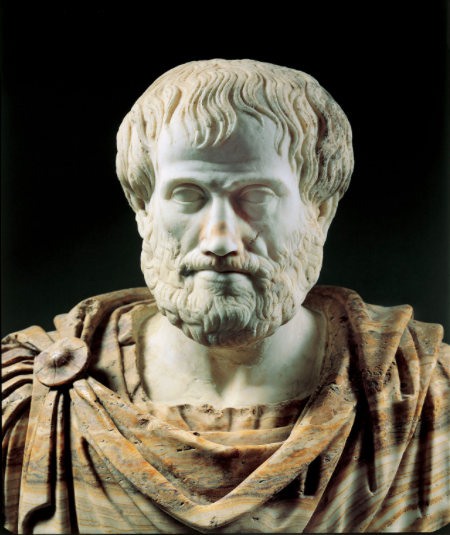
\includegraphics[width=\linewidth]{aristotle.png}}
        %Make sure the width of the picture doesn't exceed that of the box.
        \ffigbox[\linewidth]{\caption{Saul Kripke: we’ve come a long way since then.}}{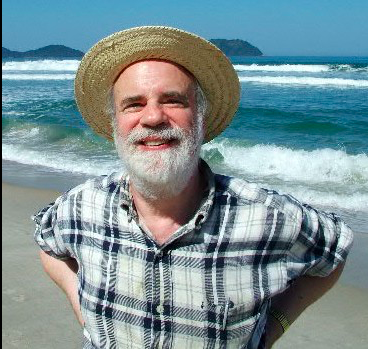
\includegraphics[width=\linewidth]{kripke.png}}
    \end{floatrow}
\end{figure}
\href{https://www.britannica.com/biography/Aristotle#/media/1/34560/76426}{Aristotle image source}\\
\href{https://commons.wikimedia.org/w/index.php?curid=5763037}{Saul Kripke image source}\\
Make sure you follow these links, so you know where the hyperlinks lead to when you typeset it yourself.
\begin{table}[H]
    \centering
    \begin{tabular}{p{10em}|p{10em}} 
        \hline
         \textbf{Assertion} & \textbf{Negation}\\
         \hline 
         $p(x)$ & $\neg p(x)$  \\
         \hline
         \multirow{2}{*}{$\perp$} & $p(x) \vee \neg p(x)$\\ %both rows with vs are combined
         & $\top$\\
         \hline
         \multirow{2}{*}{$p(x)\wedge q(x)$} & $\neg\left(p(x)\wedge q(x)\right)$ \\
         & $\neg p(x)\vee\neg q(x)$\\
         \hline
         $\exists x.p(x)$ & $\forall x.\neg p(x)$\\
         \hline
         \multirow{2}{*}{$p(x)\Rightarrow q(x)$} & $\neg\left(\neg p(x)\vee q(x)\right)$\\
         & $p(x)\wedge \neg q(x)$\\
         \hline
         \multicolumn{2}{c}{This statement is false.}\\
         \hline
    \end{tabular}
    \caption{Some First Order Logic, and an absurdity.}
    \label{tab:logic}
\end{table}
This table uses \verb!multirow! as well as \verb!multicolumn!.
Replicate it as well as you can.
\section{Maths, Theorems and References}
\begin{theorem}[Divergence Theorem]
	\begin{equation*}
		\iiint_V({\boldsymbol\nabla}\cdot\mathbf{F})dV=\oiint_S(\mathbf{F\cdot\hat{n}}dS)
	\end{equation*}
\end{theorem}
\begin{remark}
	You have definitely studied and applied the theorem extensively in MA 105.
	It also shows up as Gauss' Law in electrodynamics.
\end{remark}
\begin{proposition}[Georg Cantor]
	Let $\mathbb{N}$ be the set of natural numbers. Denote its cardinality $|\mathbb{N}|$ by $\aleph_0$.
	Let $\mathbb{R}$ be the set of real numbers.
	Its cardinality $\mathfrak{c}$ is sometimes called the cardinality of the continuum.
	$\mathfrak{c} = 2^{\aleph_0}$
\end{proposition}
\begin{hint}
	You will find the \verb!\mathfrak! command useful to typeset the above.
\end{hint}
\begin{lemma}[Jordan Normal Form]{\label{lem:jnf}}
	For every matrix $M$ in $\mathbb{C}^{\kappa\times\kappa}$ having eigenvalues $\gamma_1,\ldots,\gamma_k$ with algebraic multiplicities $m_1,\ldots,m_k$ respectively, there is an invertible matrix $P$ and a matrix $D$ of the form $D = \operatorname{Diag}(J_1,\ldots,J_k)$ with each block $J_i$ being a $m_i\times m_i$ matrix of the form
	\begin{equation*}
		J_i=
		\begin{bmatrix}
			\gamma_i & 1 & 0 & \ldots & 0\\
			0 & \gamma_i & 1 & \ldots & 0\\
			\vdots & \vdots & \vdots & \ddots & \vdots \\
			0 & 0 & 0 &  \ldots & 1\\
			0 & 0 & 0 &  \ldots & \gamma_i\\
		\end{bmatrix}
	\end{equation*}
	and $M=P^{-1}DP$. Moreover, if $M$ is an algebraic matrix, so are $D$ and $P$, and their entries can be computed from the entries of $M$.
\end{lemma}
You have certainly studied that if $M$ is defect free, that is, algebraic and multiplicities of its eigenvalues coincide, then it is similar to a diagonal matrix.
If not, the Jordan Normal form is the next best thing.
We cite \cite{book:la} for this lemma.
\begin{hint}
	Look at the bibliography entry for this citation.
	It is a book.
	Specify the author, publisher, title, year and edition.
	Our bibliography style is \verb!plainurl!.
\end{hint}
Consider the last statement of Lemma \ref{lem:jnf}. (Yes, a cross reference.)
Algebraic numbers are roots of polynomials with integer coefficients.
They can be found efficiently.
\cite{article:cma}
\begin{hint}
	This citation is an article.
	Specify the author, year, title, journal, volume and number.
\end{hint}
\bibliographystyle{plainurl}
\bibliography{references}
\end{document}